\chapter{Methods}
\label{cha:methods}
This project was part of a team effort. My contribution has been greatly influenced by other developers in our team, and the information we got were shared among us. For this reason, several aspects were a work of more than one person. In this chapter I will focus on what I personally did, but I will have to refer to work done in collaboration with others.

To share our projects and our implementations we used a GitHub organization where all our code can be found and used by others.\footnote{\url{https://github.com/WikiCommunityHealth}}

\section{Categorizing users}
\label{sec:categorizingusers}
Analyzing and making public data about a single user can be considered a violation of their privacy. We decided to group users into categories identified by their gender and role in Wikipedia and to publish only results relative to groups and not individuals.

Obtaining this information is not straightforward.

\subsection{Users' gender}
\label{sec:usersgender}
In Wikipedia, there are two main ways with which users can specify their genders: Userboxes and profile settings.

\subsubsection{UserBoxes}
\label{sec:usersboxes}
A UserBox, or UBX, is a graphical component that can be added to a user page. Some users have decided to express their gender through a corresponding UBX. There exist several genders related UBXs, grouped into 4 categories: “masculine”, “feminine”, “non-binary” and “others”.\footnote{\url{https://en.wikipedia.org/wiki/Wikipedia:Userboxes/Life/Gender}}

Thanks to Wikipedia APIs, we can list all pages that contain those templates, collecting a list of user pages, and thus usernames, that decided to express their gender as stated in the corresponding UBX.

As we will see in section \ref{sec:resuserboxes} this technique retrieved a relatively small amount of data if compared to profile settings.

\begin{figure}[H]
    \centering
    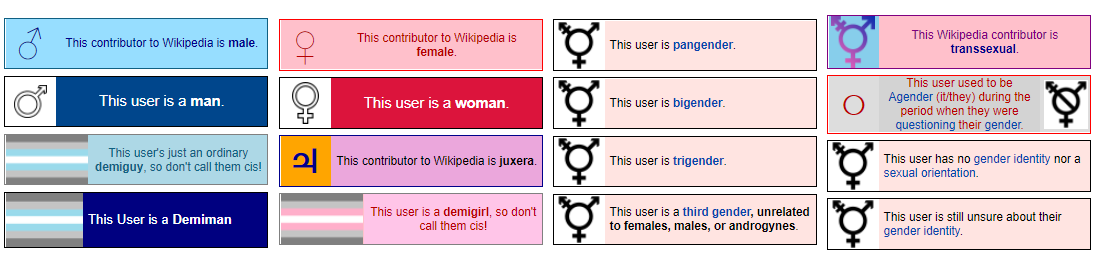
\includegraphics[width=0.85\textwidth]{./img/ubx.png}
    \caption{Examples of different UserBoxes used by the community}
    \label{fig:ubx}
\end{figure}

\subsubsection{Profile Settings}
\label{sec:profilesettings}
Each Wikipedia user has access to a settings page, where some preferences and information can be specified, including a user's gender. The user choice is restricted to “Male”, “Female” and “Unknown”, where “Unknown” is the choice selected by default when someone creates an account.

\begin{figure}[H]
    \centering
    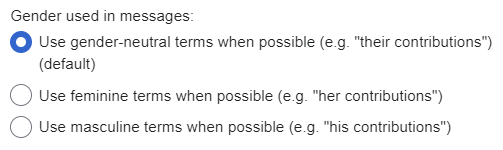
\includegraphics[width=0.7\textwidth]{./img/settings.png}
    \caption{Settings page where users can choose their gender}
    \label{fig:chainsuser}
\end{figure}

Wikipedia APIs returns a list of information about a user, among which their specified gender in the profile settings.\footnote{\url{https://www.mediawiki.org/wiki/API:Users}} We collected this and other information for all users for each language of Wikipedia.

\subsubsection{Users’ Role}
\label{sec:usersrole}
Users have been categorized based on their user groups. We considered the most common groups, which are Admins (or sysop), autopatrolled, and registered users.\footnote{\url{https://en.wikipedia.org/wiki/Wikipedia:User_access_levels}} This information has been retrieved from a dataset generated by another team member where all information about a user are collected, including their roles. Thanks to this dataset we could identify some users as a bot and remove them from our analysis.

\section{Lookup tables}
\label{sec:lookuptable}
The WikiConv dataset only provides information about actions. For our analysis, it was useful to have access to information about specific users and pages as a reference.

We decided to implement two lookup tables with basic information about each user and each page in a MongoDB instance,\footnote{\url{https://www.mongodb.com/}} a No-SQL database that stores data in JSON documents inside the collection. We choose this database because it allowed us to store and easily query our data without changing its format. To generate them, all the WikiConv dataset has been loaded into the database, then, a query, aggregated all information by the user and by page, and computed the new information seen in Figure \ref{fig:mongo}.

\begin{figure}[H]
    \centering
    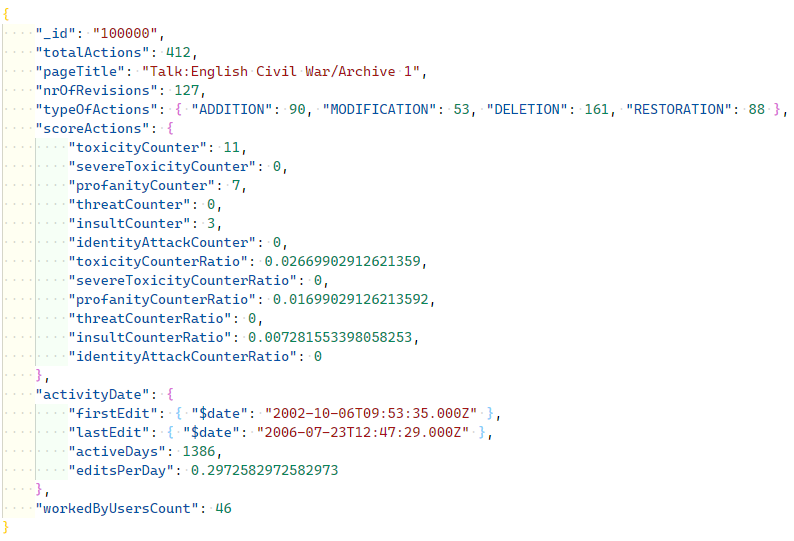
\includegraphics[width=0.85\textwidth]{./img/mongo.png}
    \caption{Examples of the document representing a Wikipedia page in the pages look-up table}
    \label{fig:mongo}
\end{figure}

\section{Sorting the WikiConv dataset}
\label{sec:sortingthewikiconvdataset}
The WikiConv dataset is composed of compressed files, each of them is about 2GB in size. Each file contains a random subset of actions of the entire dataset, and it is not possible to know in which file a specific action is contained.

We chose to sort the dataset in four different ways. Each sort is defined by a sorting feature. For each sorting feature, a set of intervals had to be chosen such that:
\begin{itemize}
\item  Each possible feature is part of one and only one interval.
\item  All intervals have a similar number of actions associated with them.
\item  All intervals are sorted such that if an interval is greater than another, then all its features are greater than the features of the other interval.
\end{itemize}

All the process was done by decompressing the file “on-the-fly”, without the need to store a plain version at any step of the process. This greatly increased performance, while reducing the storage space required for the process. The run time of the algorithm can be expressed as $O(N* M*log(M))$, where $N$ is the number of intervals, $M$ is the number of actions associated with an interval.

Of crucial importance was the choice of the dimensions of the intervals. An interval too big would result in a bigger $M$, a bigger file to sort, and thus a longer run time; whether a smaller interval would create a huge number of files to sort and a hardware bottleneck on the reading and writing performance, both during the sorting and during the analysis.

The four different sorting features are Users, Pages, Timestamp, and Reply-To.

\paragraph*{Users}
Each action can be associated with the user that made it, which can be identified by its numeric id. If an action was made by an anonymous user, no user id is saved on the dataset, but we can use its IP address to identify it. This method is not guaranteed to univocally identify a user, since many users can share the same IP address, or the same user can change IP address over time. A small set of actions had no user id and no IP address.

They were associated with a null user for the sake of the algorithm but were not analyzed after.

\paragraph*{Page}
To sort by page, we used the page id saved on each action as a sorting feature. The intervals are ranges of dimension 2 million, which covers all possible pages’ ids.


\paragraph*{Timestamp}
To sort by timestamp, we used the timestamp saved on each action. Actions from the same revision have the same timestamp, and we used their id as a secondary sorting feature since ids are ordered inside a revision. The intervals range from the start to the end of each month analyzed by the dataset.

\paragraph*{Reply To}
The reply to is a field that is not present in the original dataset. It was computed by another team member, by reconstructing the discussion tree of each page and assigning as “reply to”, the id of the user that the action was addressed to. This field is useful to understand which emotions are addressed to which user.

The intervals we used are the same as the ones we used for the user id.


\begin{table}[H]
    \centering
    \ra{1.2}
    \begin{tabularx}{\columnwidth}{@{}Xrrrr@{}}
        \midrule
        \textbf{Language} & \textbf{Lines} & \textbf{Size} & \textbf{Compressed size} & \textbf{Time to sort}\\ \toprule
        English & 235 Millions & 485 GB & 129 GB & 12 h \\
        Spanish & 20 Millions & 41 GB & 11 GB & 1:30 h \\
        Italian & 17 Millions & 41 GB & 11 GB & 1:30 h \\
        Catalan & 2 Millions & 7 GB & 2 GB & 0:30 h \\

         \bottomrule
    \end{tabularx}
    
    \caption{The table shows the number of actions in each dataset, the size of the compressed and uncompressed dataset and how much it took to compress.  \label{table:datasetsize}}
\end{table}


\section{Minifying the WikiConv dataset}
\label{sec:minifingthewikiconvdataset}
The WikiConv contains a lot of information that is not used during our analysis. We choose to generate a new parsed dataset containing only the information we needed. For each action, we kept id, action type, page title and id, username and id, and timestamp. The text content was parsed into an array of integers, where each integer is the number of words in the text associated with an emotion according to the lexicon dictionary.

Analyzing these versions of the dataset was much faster since the words were already associated to an emotion, and thanks to the reduced size of the file. It was also simpler to move and store the files.

\begin{figure}[H]
    \centering
    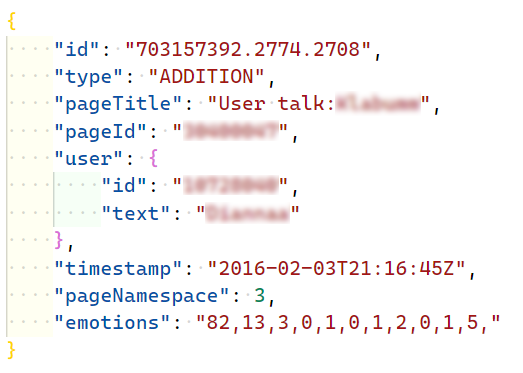
\includegraphics[width=0.6\textwidth]{./img/min.png}
    \caption{Examples of the document representing an action in a minified dataset}
    \label{fig:min}
\end{figure}


\begin{table}[H]
    \centering
    \ra{1.2}
    \begin{tabularx}{\columnwidth}{@{}Xrr@{}}
        \midrule
        \textbf{Language} & \textbf{Sorted dataset size} & \textbf{Minified dataset size} \\ \toprule
        English & 81 GB & 3.2GB  \\
        Spanish &  6.8 GB & 0.32 GB \\
        Italian &  6.1 GB & 0.30 GB \\
        Catalan &  1.4GB & 0.04 GB \\

         \bottomrule
    \end{tabularx}
    
    \caption{The table shows the difference in size from the sorted dataset to the minified dataset. \label{table:datasetsize}}
\end{table}


\section{Analyzing the WikiConv dataset}
\label{sec:analyzingthewikiconvdataset}
All the analysis tools have been written in Python 3.\footnote{\url{https://www.python.org/}} Python is an interpreted programming language suited for data science. It has a plethora of useful libraries for the tasks we are interested in and offers great flexibility.

We developed a python module that offers a command-line interface to allow a user to analyze either the sorted WikiConv dataset and the minified sorted WikiConv dataset. Through dependencies injection, the module can load an “analyzer”: a service that offers some APIs for the module to compute a different kind of analysis.

The module computes several tasks. Firstly, it reads a specified set of files, decompressing them on the fly, if necessary. Then it goes through all actions in the file, grouping them by their sorting feature. Since the sorting feature is sorted, once a different feature is read, the previous group is completed and can be passed as input to the analyzer which does its specific computations and remove from memory. The module also handles parallelization running each file in a different thread. The user can specify if he wants to use parallelization and the maximum number of parallel threads running.

An analyzer handles every possible analysis. They can be developed independently but need to implement a set of APIs called by the module. They are used to pass the actions groups and to synchronize the progress among different threads.

We developed several analyzers to handle different tasks, the important ones are described here:

\paragraph*{Minifier}
This analyzer allowed us to reduce the dataset structure as described in section \ref{sec:minifingthewikiconvdataset}. It took each line, calculated its minified version, and generated the new file version.

\paragraph*{Reply To}
It was used to create a new feature in the dataset called “replyTo” described in section \ref{sec:sortingthewikiconvdataset}. This feature identifies which users are an action addressed to.

\paragraph*{Reply To}
Mean and Var Analyzer:	It analyzed the mean and variance of emotions in each activity group. The output is a JSON file containing the total mean and variance of each emotion contained in the analyzed text and the number of actions analyzed. The results were also calculated and saved for each month contained in the action group. This gave us global information about a user or a page through time. It was also possible to use this analyzer to compute the same information for the whole dataset, giving us a reference point and a view of the whole Wikipedia in a particular month.

\paragraph*{Word Cloud}
Word Cloud:	This analyzer created a graphical representation of the most used words by a user, by a page, in a month, or Wikipedia as a whole. Seeing what words, the lexicon analyzed and associated with different emotions was difficult to verify manually, and having a graphical representation of its work was useful. It was used to verify and validate our works and the dataset we used and to illustrate our works to others simply and effectively.

\paragraph*{Emotions to DB}
This analyzer reads all emotions and generates the metrics to add to a Postgres database. We created metrics about pages and users’ groups for any month in the dataset. These metrics were saved in a SQL database and were then published.

\paragraph*{Emotions to JSON}
This analyzer, similarly to “Emotion to DB”, generates metrics about users’ groups and pages, but saves them in a JSON file. This is mostly used to rapidly share information among team members and is used as input for other scripts, such as the one that draws the charts.

\paragraph*{Emotions to CSV}
Similarly, to “Emotions to DB” and “Emotions to JSON”, this analyzer generated metrics about users’ groups and pages in CSV. These files were used by a researcher to develop a project of data visualization. We choose to use CSV since it is a simple and straightforward file format, that can be used without any special technical abilities.


\section{Metrics}
\label{sec:metrics}
Metrics are the core result of this study. They can be used to characterize users and pages by their emotions and can be exported and incorporated into other projects. It is important to make all metrics useful on their own and should be compared with each other. Each team member had different metrics and different approaches to compute them, but we tried to make them as similar as possible following this guideline:

\begin{itemize}
\item  Each metrics value should refer to a users’ group or a page
\item  Each metric value should refer to a month
\item  For each metric value there should be three linked metrics:
\begin{itemize}
\item  \textbf{Normalized}: the value normalized with a set of other metrics
\item  \textbf{Accumulated}: the current month metric value summed to all the same metrics of the previous months.
\item  \textbf{Accumulate Normalized}: the accumulated value normalized in the same way the normalize value was calculated.
\end{itemize}
\end{itemize}

To facilitate this process a Python package was developed, with the help of a team member. It helps our team members to format the metrics to follow our guidelines and push them into a database. The package can be installed via pip in any Python 3 project.

